A Figura~\ref{fig:comparacao_aleatoria} apresenta a comparação entre
os sete algoritmos implementados (os seis algoritmos estudados, sendo o
\textit{Quick Sort} em suas duas versões) para entradas geradas
aleatoriamente.

\begin{figure}[H]
    \centering
    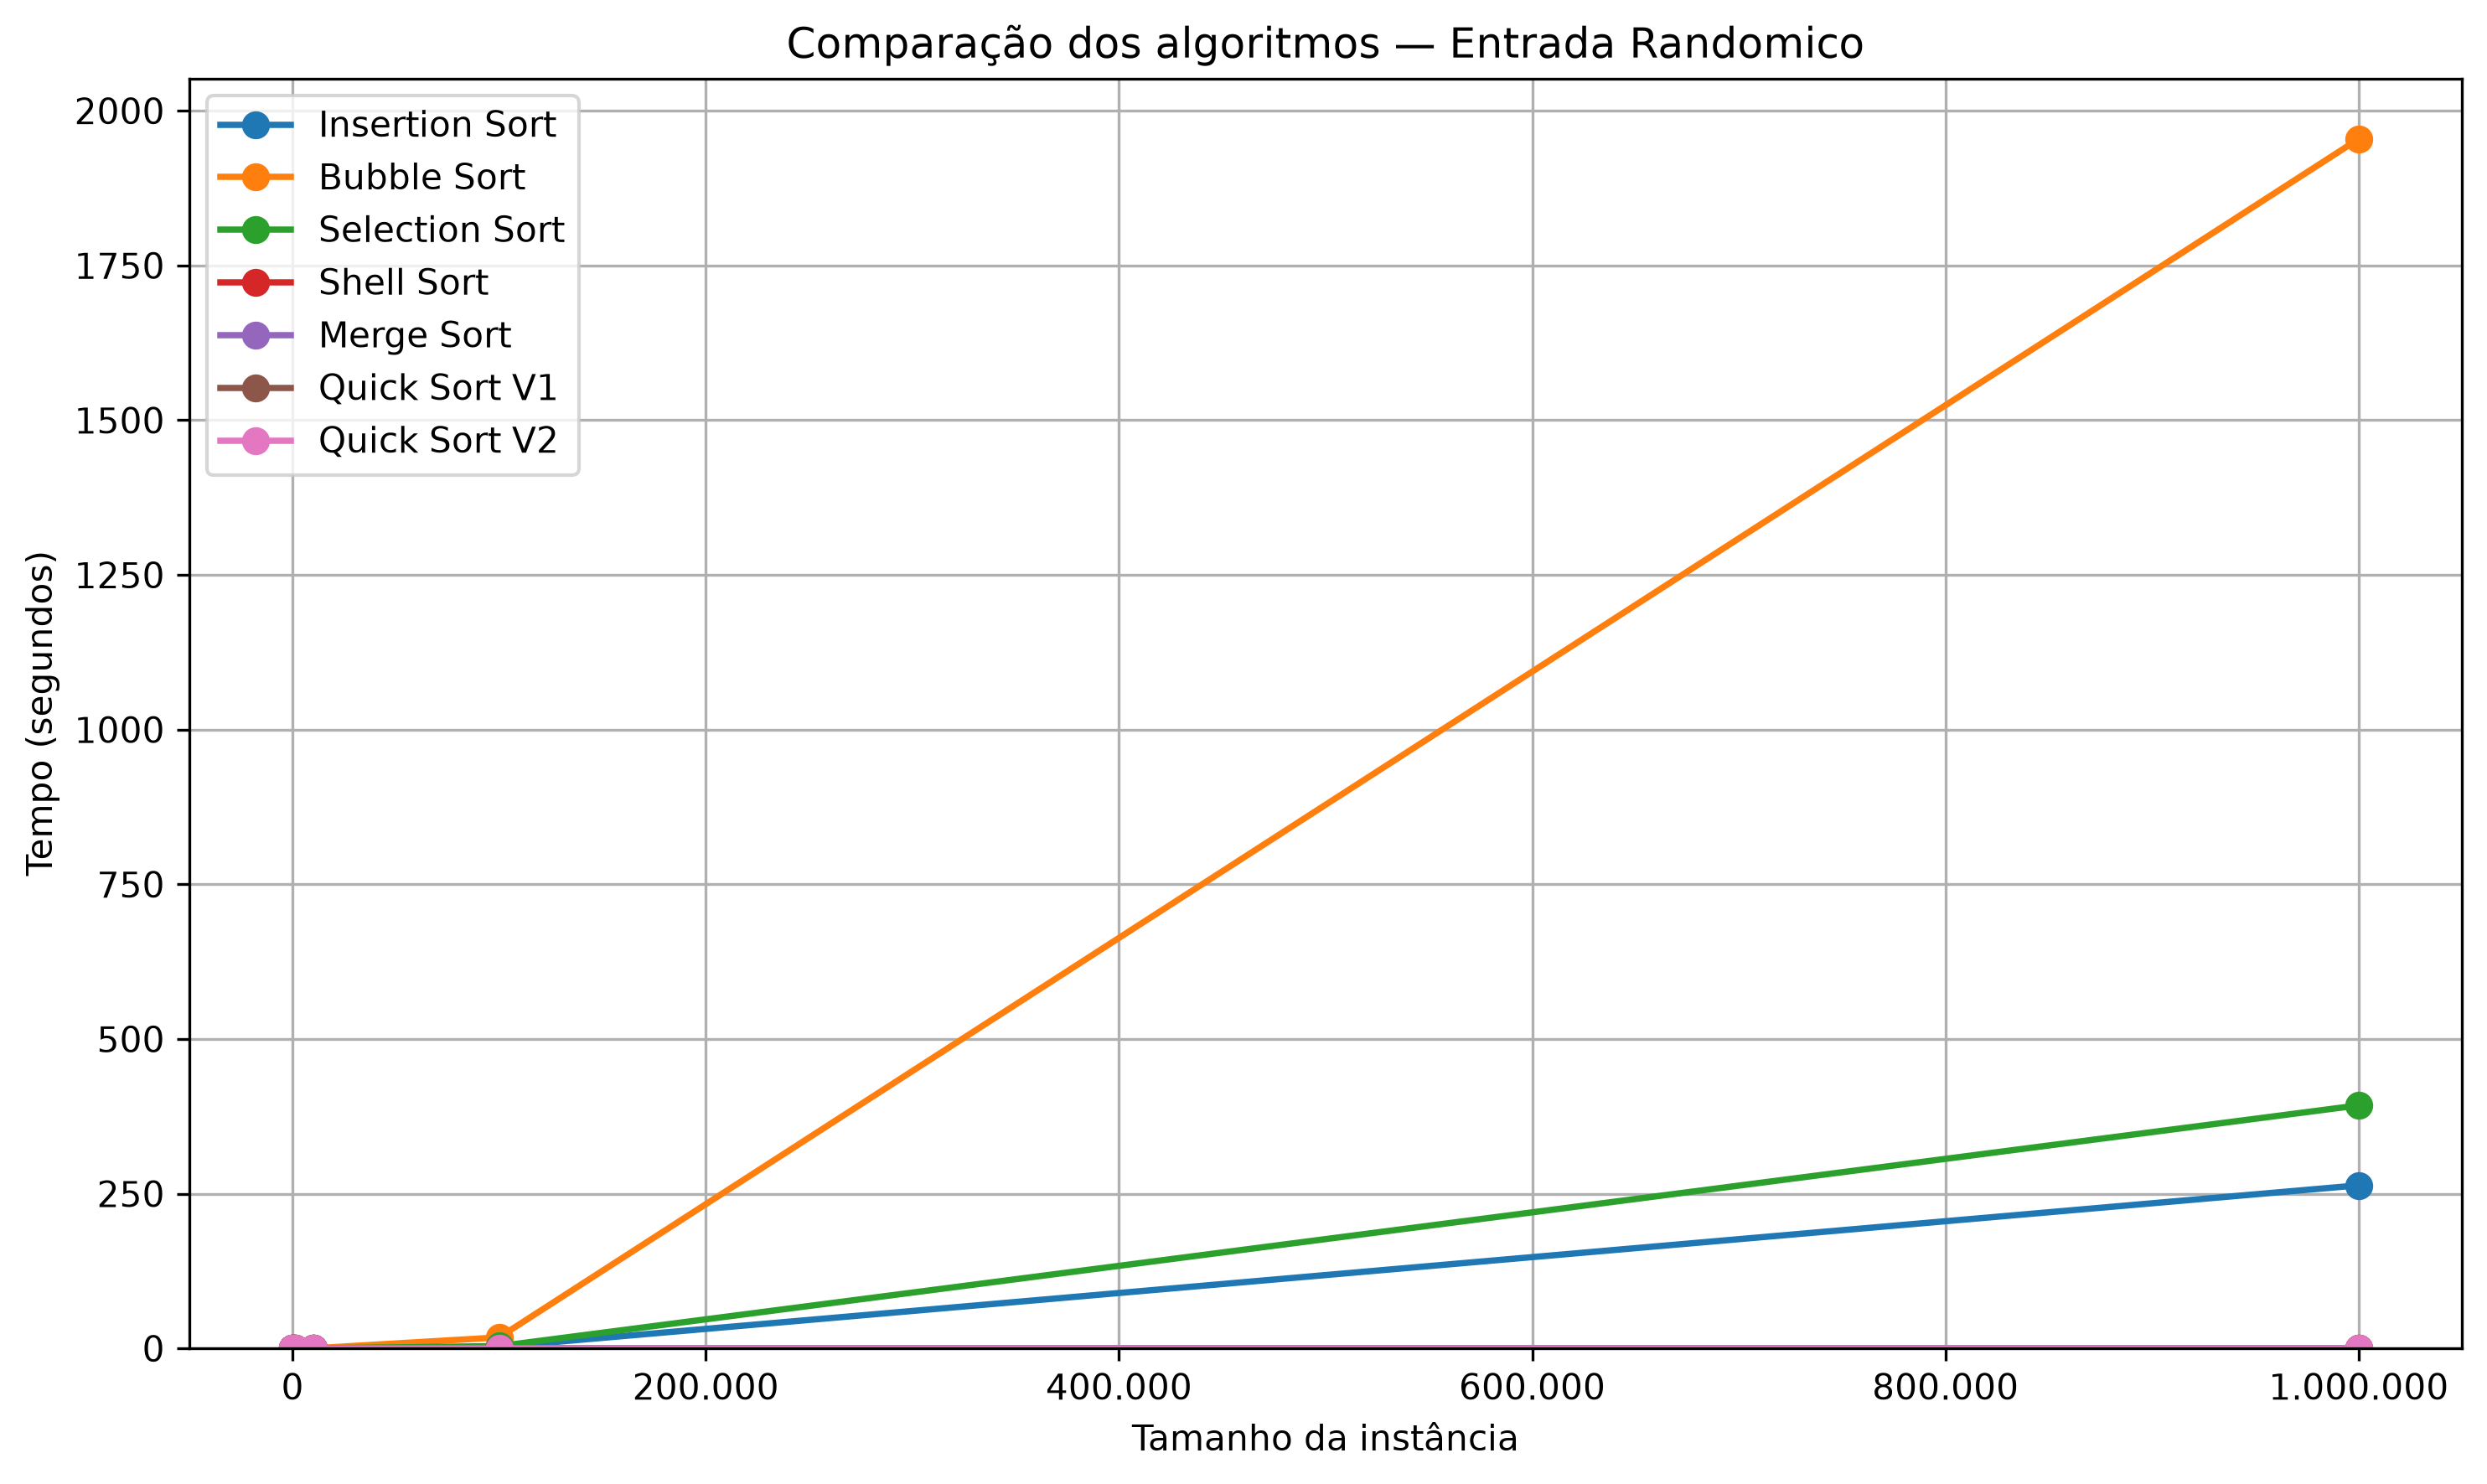
\includegraphics[width=\textwidth,keepaspectratio]{Imagens/Comparacoes/comparacao_aleatoria.png}
    \caption{Comparação dos algoritmos para entrada aleatória.}
    \label{fig:comparacao_aleatoria}
\end{figure}

Para as entradas aleatórias, observa-se uma separação clara entre os
algoritmos de custo quadrático e os demais. Para instâncias de
1.000.000 de elementos, o \textit{Bubble Sort} apresenta o maior tempo
de execução, em torno de 1950 segundos, seguido pelo \textit{Selection
Sort}, com cerca de 390 segundos, e pelo \textit{Insertion Sort}, com
cerca de 260 segundos. Esses resultados são coerentes com o crescimento
quadrático esperado no caso médio. A menor quantidade de deslocamentos do
\textit{Insertion Sort} em relação às trocas do \textit{Bubble Sort}
explica a diferença entre eles, mesmo com a mesma ordem de complexidade.

O \textit{Shell Sort}, o \textit{Merge Sort} e as duas versões do
\textit{Quick Sort} apresentaram tempos muito inferiores aos dos
algoritmos quadráticos, praticamente indistinguíveis do eixo horizontal
na escala do gráfico. Isso confirma, na prática, a vantagem dos
algoritmos com custo próximo de $\Theta(n\log n)$ para instâncias
grandes. No caso do \textit{Quick Sort}, as duas versões apresentaram
comportamento semelhante em entradas aleatórias, pois, nessa situação, o
primeiro elemento e a média aritmética tendem a gerar partições
razoavelmente equilibradas.
